\chapter{Model specifications} \label{ch:model_specs}

This chapter presents the physical aspects of the snake robot model used throughout the report. The model has three main parts, namely the environment, the snake robot and the obstacles. The value of all variables needed to express the model and control goals are assumed known at all times. Further assumptions are presented below. This chapter is taken from the previous work of the author \cite{AtussaProsjektoppgp}, but some of the assumptions are modified to conform with the current project.

\section{Assumptions}\label{seq:assumptions}

Assumptions 1-6 are taken from Stavdahl \cite{StavdahlNote}, whilst assumptions 7-9 are specific for this project.

\begin{enumerate}
    \item All parts of the model are assumed to be rigid.
    \item The robot has $n$ joints and all links have length $l$ and mass $m$.
    \item Only flat, 2-dimensional cases are considered.
    \item The robot has no lateral extension.
    \item There is no friction. 
    \item Obstacles have no spatial extent, only a static position in the plane.
    %\item During an impact with an obstacle, the configuration of the snake robot, $\mathbf{q}$, remains unaltered while the velocity, $\mathbf{\dot{q}}$, will generally experience a jump.
    \item Any link is in contact with at most one obstacle at the time.
    \item The robot is in touch with obstacles in its start configuration.
    \item Contact between a link and an obstacle is maintained.
\end{enumerate}

%----------------------------------------------------------------------------------
%----------------------------------------------------------------------------------

\section{Further model description}

\subsection{The snake robot}
The snake robot itself is modeled as a simple planar robot manipulator with links and joints. The main difference between the snake robot and a classic robot manipulator is the property that the snake robot is not physically attached to any fixed point in the world. This frees one constraint. However, it is still relevant to express the position of the first link of the snake, also denoted as the tail. This is performed by introducing three virtual joints to the model; two translational and one rotational joint. These joints are not controllable and merely for describing the kinematics, dynamics and constraints. The model of the snake robot is visualized in Figure \ref{fig:2_kin}, where physical robot links are blue and the virtual ones are green.

\begin{figure}
    \centering
    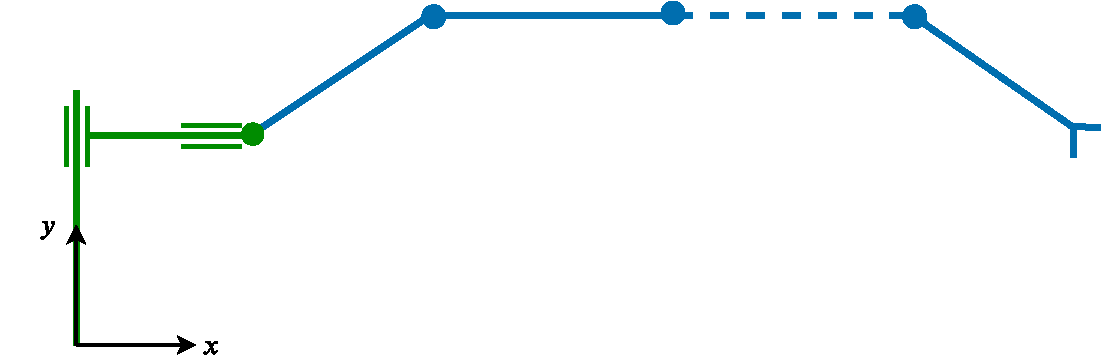
\includegraphics[width=0.9\textwidth]{figures/modelspecs/superbasicsnake.pdf}
    \caption{Model of snake robot with $n$ links}
    \label{fig:2_kin}
\end{figure}

%----------------------------------------------------------------------------------
%----------------------------------------------------------------------------------

\subsection{The environment}
The environment is the (x,y)-plane in Figure \ref{fig:2_kin}, and consists of nothing but the robot and the obstacles.

%----------------------------------------------------------------------------------
%----------------------------------------------------------------------------------


\subsection{The obstacles}

The obstacles are modeled as rigid points in the plane and any contact with them is considered a point contact. Figure \ref{fig:2_kin_obst} shows three obstacles in contact with a snake robot.

\begin{figure}[h!]
    \centering
    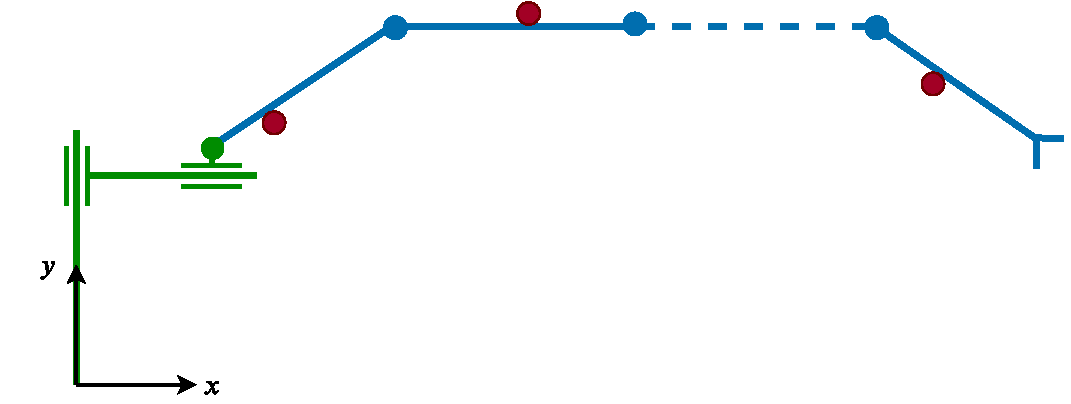
\includegraphics[width=0.9\textwidth]{figures/modelspecs/superbasicsnakenobstacles.pdf}
    \caption{Model of snake robot and obstacles}
    \label{fig:2_kin_obst}
\end{figure}
